% Intended LaTeX compiler: pdflatex
\documentclass[10pt,a4paper,UTF8]{article}
\usepackage{zclorg}
\usepackage{tikztheorem}
\author{zcl.space}
\date{}
\title{Distance}
\hypersetup{
 pdfauthor={zcl.space},
 pdftitle={Distance},
 pdfkeywords={PMA},
 pdfsubject={},
 pdfcreator={Emacs 25.0.50.1 (Org mode 9.1.2)},
 pdflang={English}}
\begin{document}

\maketitle
\tableofcontents
\titlepic{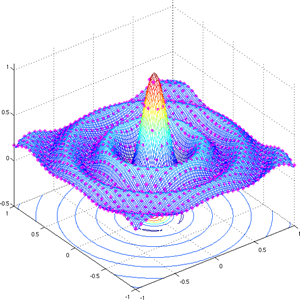
\includegraphics[scale=0.25]{../../img/sinc.PNG}}
The \textbf{distance}  \(d(p,q)\) between two points \(p=(x_1,x_2,\ldots,x_n)\)
and \(q=(y_1,y_2,\ldots,y_n)\) in \(\mathbb{R}^n\) is  defined by\footnote\{
In Chapters I-V Buck  writes \(|p-q|\) instead of \(d(p,q)\) but
uses  the notation \(d(p,q)\) starting in Chapter\textasciitilde{}VI  (page\textasciitilde{}304) in
a more general setting.\}
$$
 d(p,q)=\sqrt{(x_1-y_1)^2+(x_2-y_2)^2+\cdots+(x_n-y_n)^2}.
$$
The distance \(d(v,0)\) from a vector \(v\in\mathbb{R}^n\) to
the origin is  called the \textbf{norm}  of \(v\) denoted by \(|v|\) so
$$
      d(p,q):=|p-q|.
$$
The norm satisfies the following laws for \(v,w\in\mathbb{R}^n\):

\begin{enumerate}
\item \textbf{zero norm}  \(|v|=0\iff v=0\),
\item \textbf{homogeneity} \(|av|=a\,|v|\) if \(a>0\),
\item \textbf{symmetry} \(|-v|=|v|\),
\item \textbf{triangle inequality} \(|v+w| \le |v|+|w|\).
\end{enumerate}

The zero norm law holds  because a sum of squares vanishes

The laws for the norm imply that
the distance function satisfies the following:

\begin{enumerate}
\item \textbf{zero distance} \(d(p,q)=0\iff p=q\),
\item \textbf{symmetry} \(d(p,q)=d(q,p)\),
\item \textbf{triangle inequality} \(d(p,r)\le d(p,q)+d(q,r)\).
\end{enumerate}

These are proved by reading \(v=p-q\) and \(w=q-r\) in the corresponding
law for the norm.


  Define the \textbf{inner product}  of two vectors in \(\mathbb{R}^n\)
by
$$
    \langle u,v \rangle =u_1v_1+u_2v_2+\cdots+u_nv_n
$$
for \(u=(u_1,u_2,\ldots,u_n)\), \(v=(v_1,v_2,\ldots,v_n)\). In freshman calculus you called this the \textbf{dot product}
and learned that the angle \(\theta\) between the two vectors \(u\) and \(v\) satisfies
$$
    \langle u,v \rangle =\cos\theta\,|u|\,|v|.
$$
Since the cosine takes values between -1 and +1, it follows that
\begin{equation}
\label{eq:1}
    |\langle u,v \rangle | \le |u|\,|v|.
\end{equation}

This inequality is called the \textbf{Schwarz inequalityr}.



For \(p\in\mathbb{R}^n\) and \(\delta>0\) the set
$$
    B(p,\delta):=\{q\in\mathbb{R}^n:d(p,q)<\delta\}
$$
is called the \textbf{open ball}  centered at \(p\) with radius \(\delta\).
When \(X\subseteq\mathbb{R}^n\) we often use the abbreviation
$$
    B_X(p,\delta):=B(p,\delta)\cap X:=\{q\in X: d(p,q)<\delta\}
$$

When \(n=1\) the open ball is an open interval:
\begin{eqnarray*}
 B(a,\delta)&=&\{x\in\mathbb{R}: |x-a| < \delta\}\\
            &=&\{x\in\mathbb{R}: a-\delta < x < a+\delta\}\\
            &=&(a-\delta,a+\delta)
\end{eqnarray*}
for \(a\in\mathbb{R}\)


 A set \(S\) is \textbf{bounded}  iff it is contained
in some large ball, i.e. iff there exists \(M>0\) such that
\(|p| < M\) for all \(p\in S\). Thus a set of real numbers
is bounded if and only if it is bounded above and bounded below.
\end{document}